% introduction.tex

\section{Introduction}
Voldemort is an implementation of a distributed, highly available key-value store.
The configuration of the system is however cumbersome and tedious, so we would like to explore the possibilities for using ZooKeeper to coordinate configuration and later some management tasks.
Such tasks includes extending and reducing the members of the cluster.

We have created a method for managing cluster metadata and configuration for Voldemort by using Apache ZooKeeper for coordination.

In this process we have implemented an internal StorageEngine that uses ZooKeeper for node configuration and metadata.

We have also implemented a service, named Headmaster, that manages configuration, node discovery and node membership in the cluster.
Headmaster can also decide whether to execute a rebalance based on certain criteria.

\subsection{Voldemort and Dynamo}
Voldemort is a software system based off of Amazon's paper on Dynamo, Amazon's highly available key-value store\cite{dynamo}.

The supported queries are limited to simple get and put operations on objects uniquely identified by a key. 
The objects stored are by the system considered binary blobs.
The database is mainly used to store lots of smaller items, typically less than 1MB in size.

\subsubsection{Motivation for these systems}
Traditional relational database systems are generally very safe to use, usually providing all of the ACID (\emph{Atomicity, Consistency, Isolation, Durability}) properties.
This guarantees that all committed transactions are processed reliably.
Experience has however shown that databases providing ACID guarantees have trouble scaling. It is very difficult, if not impossible, to have ACID databases handle the high traffic volumes in addition to the high availability demands of today.

Voldemort and Dynamo sacrifices consistency and isolation requirements to achieve higher availability with satisfactory durability.
In fact, we will later see that most of this behavior is easily tunable and left as design choices per implementation.
You should also note Voldemort (and Dynamo) does not guarantee any form of isolation and does not support multiple key updates.

\subsection{Techniques and technologies}
The software used in this project employ many different and important techniques known from distributed computing, and will be discussed here.

\subsubsection{PAXOS}
Whenever you have a distributed system where errors occur and messages get lost, even simple tasks like deciding on a value can become troublesome. Paxos an consensus algorithm made to solve this issue. 

Say we have a set of processes that all can propose values. (The value could be related to leader election). Paxos ensures that a single one of these values is chosen and that all processes involved is notified of this value. If no value is being proposed, then no value should be chosen. 

In Paxos a process can act in three different roles: {\it proposer, acceptor and learner}. A process is not limited to one role at the time. Processes communicate with one another by messages. These massages follow the non-Byzantine model and can take arbitrary long time to be delivered, or they can be lost entirely. They can also be duplicated, however they can not be corrupted. A process acting in a role might also crash, but we assume some critical information will remain through a restart. 

When acting as a proposer, a process will propose a value to a majority subset of acceptors. These acceptors will then accept or deny the proposal according to some rules. Finally if a value is chosen, then all the learners will be informed of this value. This is the process of choosing a value:

\begin{enumerate}

\item A proposer sends a prepare for proposal message to a majority set of acceptors with a number n. This number works like a time stamp represent the last(newest) message this proposer has seen. 
\item Each acceptor receiving this prepare for proposal message will compare this number n with their own highest observed n. If the proposed number is higher, then a promise of not accepting any proposal lower than n will be sent back to the proposer along with the acceptors highest observed value. If the proposers number is lower than the acceptors observed number, then the value will simply be sent back. 
\item If the proposer received a promise from majority of acceptors it will send an accept message to the acceptors with the number n along with the value v which is the maximum values received from the acceptors. If the number of promises is less than the majority of acceptors then the attempt has failed, and the proposer must start again with a higher number n.
\item When an acceptor receives an accept massage it will accept this proposal as long as there has not been issued a new proposal with a higher number in the meantime. 
\item Finally, when an acceptor has accepted a proposal it informs all learners. Either by sending a massage to all learners, or by sending a message to a designated learner, which in time will inform all other learners. This second step reduces message load but is less reliable.

\end{enumerate}

It is possible to construct a scenario where two proposers keep out proposing each other and no progress is ever made. To combat this a distinguished proposer must be elected. 

Paxos can typically be used in distributed systems to coordinate processes. One example is leader election.




\subsubsection{Consistent hashing}
\label{sec:consistenthashing}
Consistent hashing is a technique introduced in 1997 by David Karger et al.\cite{Karger97consistenthashing}
The technique is used to solve problems with locating a key in a distributed system.
Let's assume you have $n$ servers in the system, then number these from $0$ to $n-1$.
The hashspace of the keys are then divided into $n$ partitions. Then do a $\textrm{Hash(key) mod } n$ and you have the server location for the key.

However, with this scheme if a server fails and you now have $n-1=m$ servers, all the failed server's data is gone.
You have to invalidate all existing servers, renumber your set of servers and start over.

Consistent hashing reduces this problem by assigning each node with a number of points in the hash space.
The hash space is viewed as a ring by wrapping around \texttt{0000-FFFF}. The nodes are placed at points along the ring as in Figure \ref{fig:hashring}. When a key is looked up, you find it's place on the ring and move clockwise to the first point with an assigned node. In Figure \ref{fig:hashring}, key K is routed to the next node on the ring, node B.

Now remember we let the nodes take on \emph{several} points along the ring, thus spreading a nodes responsible key space to smaller pieces along the ring.
I.e. nodes B, E and G in Figure \ref{fig:hashring} could be the same \emph{physical} node.

\begin{figure}[h]
    \centering
    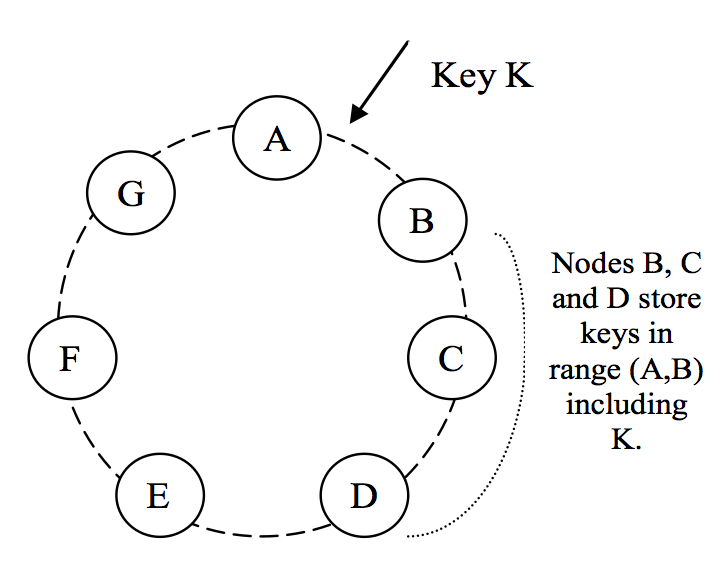
\includegraphics[width=0.5\textwidth]{introduction/hashring}
    \caption{Hash ring with several nodes\cite{dynamo}.}
    \label{fig:hashring}
\end{figure}

This approach to locating keys has several advantages:

\begin{itemize}
\item Like before, we distribute operations on the set of available servers. By having each server take numerous positions on the hash ring, we also gain a more even distribution of the amount of key space among the nodes, compared to giving them a single random or fixed position.

\item Consistent hashing can also accommodate different types of servers by allowing more powerful nodes to have more points assigned on the ring, and vice versa. 

\item When adding a new server, a number of different areas around the circle are affected, and not one contiguous piece. This means the work of adding in the new node will be spread over the system, and not all requests routed to a single node.

\item The spread of the key space also avoids rehashing of more than $k/n$ keys when adding a new node. 

\item When a node fails, you move along the ring to the next server. When the nodes occupy several points on the ring, the extra work because of a failing node will be distributed among all the nodes in the system.
\end{itemize}

Consistent hashing also conveniently allows for easy, tunable replication of data to ensure durability, as used by key-value stores Dynamo\cite{dynamo} and Voldemort\cite{voldemort}. Consider W the number of data replicas to create. Hash the key, then move along the ring, writing key K to the W first nodes encountered on the ring. This will also ensure backups to be available along the ring when a node fails and requests gets passed along.

\subsubsection{Durability}
As explained in \ref{sec:consistenthashing}, both Voldemort and Dynamo use consistent hashing to locate and and store keys.
They are both key-value stores only.
The goals for the Voldemort project is a database which is highly available and fault tolerant, providing an \emph{always-on} experience.

To allow for safely storing user data, redundancy is required. 
The typical approach to this is synchronously storing replicas at different locations to ensure data replication. 
In practice though, providing this kind of strong consistency in a database system can prove detrimental to availability in some failure scenarios.
A common approach to failure is locking down data and making it unavailable until the failure is resolved, so as not to serve potentially stale or erroneous data.
While this is very convenient for the programmer, it is not ideal for performance.
In distributed systems network and system failures can be quite common, making strong consistency very costly. In practice, strong consistency can be considered incompatible with high availability.
This makes traditional replication guarantees unsuitable for highly concurrent distributed systems.

\begin{wrapfigure}{R}{0.5\textwidth}
    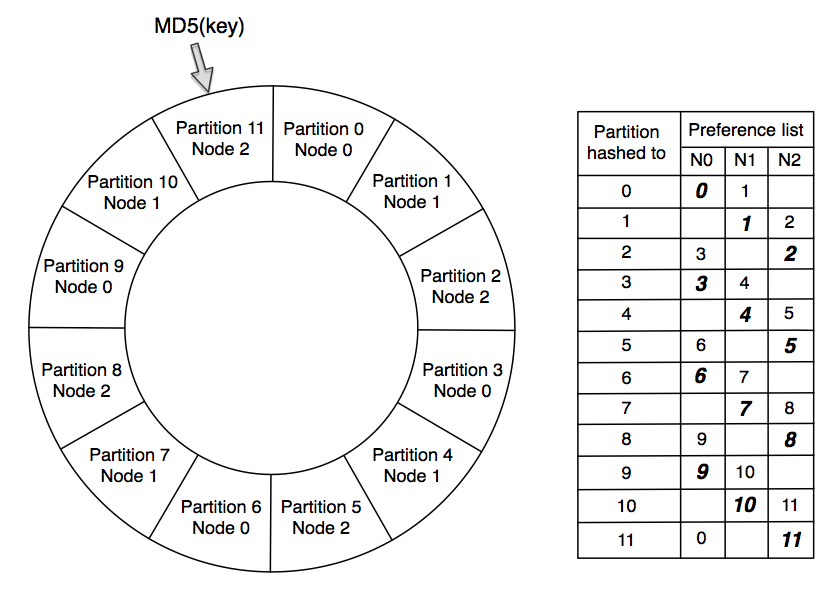
\includegraphics[width=0.5\textwidth]{introduction/hashring_voldemort}
    \caption{Hash ring with 3 nodes and 12 partitions from Voldemort\cite{dynamo} with N=2. Partitions are a fixed number of splits of the keyspace. Nodes are assigned a number of partitions which they hold. When a request is routed, one first hashes the key to find the partition the key belongs on. One then asks nodes in the order of the \emph{preference list} for the key.}
    \label{fig:voldemort_hashring}
\end{wrapfigure}

To help provide higher availability of data, an optimistic approach to replication is used.
By allowing replicas to gradually propagate in the background and not synchronously, the workload on a distributed database system is greatly relieved, allowing for higher throughput. By also allowing conflicting data, we can continue to serve data in times of failure. This will cause more work for the application developers, and they need to be aware of this when using the database. Allowing conflicts also helps availability of put operations, and allows us the possibility to always accept a write.

It is easy to see how the consistent hashing ring helps implement this approach in Voldemort.
To ensure data durability, one can simply write the data to the next few nodes on the ring. In Dynamo and Voldemort this is a tunable parameter, W, which controls how many nodes a write synchronously has to reach to be successful. 
Internally it is called \emph{required writes}.

Similarly, it is easy to see how we can implement optimistic replication.
By allowing nodes to push written object in the background at a later time to any number of nodes further down the ring.
This number \emph{N}, is called the \emph{replication factor}, and designates the number of replicas we \emph{eventually} want to be present.
I.e. we will have an \emph{eventually consistent} form of replication.

You should also note that this replication has two benefits: 
\begin{itemize}
	\item As a data backup should the other node have a hard drive failure
	\item As a functional backup. If the other node is off line, the replica can take over the workload with all the data available.
\end{itemize}

In Voldemort, the hash ring is split into X equally sized parts, called \emph{partitions}. Each partition is assigned a unique ID and maps to a node.
The nodes create a \emph{preference list} over the partitions, which says to which \emph{partitions} it should store the replicas.

Now let N=2 with 12 partitions as in Figure \ref{fig:voldemort_hashring}. 
Let a key K hash to belong in partition 0. From the preference list, we see that this key should be put in \texttt{node0}, and replicated to the node holding partition 1, which is \texttt{node1}.
Voldemort also does some sanity checking when replicating, such that replicas are always replicated to N \emph{physical} nodes. 
I.e. In our example, if both partition 0 and 1 where held by \texttt{node0}, Voldemort would move along the ring until it finds the next partition that is assigned to a different node before storing the replica.

\subsubsection{Dealing with data conflicts}
Introducing optimistic replication to increase availability of the system, even in cases of nodes being unavailable has it's price. 
In a distributed system nodes can be unreachable for a number of reasons.
Network splits, nodes dying, overloaded network and concurrent operations (remember no isolation or locking) may introduce conflicts in the data set.
These conflicts need to be discovered and resolved at some point.

Deciding how to deal with conflict is an important decision.
The questions of when to resolve them and who should have the task of doing so all have different properties.
A traditional approach is to resolve conflicts when they appear, i.e. on writes. 
This has the benefit of keeping read logic simple, but we may have to reject a write if not all (or a majority of) replicas are reachable. Resolving conflicts on write is also easy for the user to reason with.

Voldemort however wishes to run an always writable store. No data write should fail as far as we can, even during network splits and failing nodes.
This requirement makes it impossible to resolve conflicts on write, and forces us to do conflict resolution on read.

This leaves the question of who should resolve the conflicts. We can either let the database store do conflict resolution or leave it to the application.
If the store itself is going to resolve conflicts, it's choices in doing so are relatively limited.
The store can not include domain knowledge for every possible application, so it can only do simple choices like last write wins or append the difference (which isn't even resolved, and probably destructive to the stored data). Recall that to the store most of the values are considered binary blobs.

The application however has intricate knowledge of the data and is in a much better position to make good decisions. 
Amazon\cite{dynamo} uses their shopping cart as an example. If two writes are two different products added to a shopping cart, we can record both of the writes even if they are divergent.
Then at read, the application can use both versions to create a new cart with both products in it, i.e. merge the changes in a reasonable way, and present them to the user.
This requires a bit of work from the developer, which they may not want or need to do, so there is also the option of doing simple conflict resolution on the server.

\begin{wrapfigure}{r}{0.5\textwidth}
    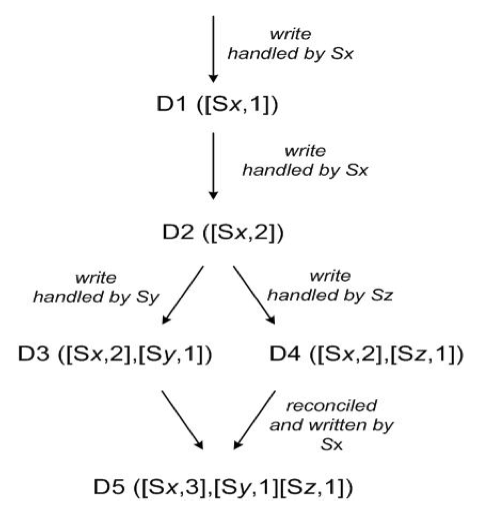
\includegraphics[width=0.5\textwidth]{introduction/versioning}
    \caption{Hash ring with 3 nodes and 12 partitions from Voldemort\cite{dynamo} with N=2.}
    \label{fig:versioning}
\end{wrapfigure}

To be able to record all changes (writes), Voldemort uses a versioning system to record the history of all changes. The data are immutable blobs, and each write creates a new version with a history of predecessors.
To record this version history, Voldemort employs \emph{vector clocks}.

Roughly vector clocks are implemented as a list of \texttt{(node, counter)} pairs and this list is stored with every version of every stored object.
By evaluating the vector clocks between two versions (or more), we can decide if one follows the other or not. If \texttt{one} followed as a version of \texttt{two}, we can discard \texttt{two} and use \texttt{one} because the changes for two are already included in this object. If the histories are divergent, we have a conflict and need to do some sort of merge or resolution.

Every time a write happens, we increment the version counter for the node who recorded the write, creating a full version history.



To facilitate the high demand for availability, Voldemort and Dynamo always allow writes.


vector clocks

\subsubsection{Membership}
In a distributed system individual nodes sometimes need to know what other nodes are available in the system. We call this group membership. Whenever a node crashes we want its membership removed so that other nodes are aware of the crash. This can be achieved in various ways. 

\begin{itemize}
\item A central service where nodes register themselves and send keep alive messages to verify that they are alive. When a new member is added or removed the service can simply broadcast a message to all members of the change. A drawback of this strategy is that we now have a single point of failure as well as a solution that does not scale very well. As nodes increase traffic into the central controller will increase as well. ZooKeeper can be used as one such central service as will be explained in the ZooKeeper section.
\item The Gossip Protocol is a peer-to-peer version. It is modeled after how information spreads in social networks. By having nodes pair up with random partners at a given intervals and exchange information we allow this information to spread throughout the system. This allows the system to reach an eventual consistent state without having any single broad-casted message. To add a node to the group simply pair it with one existing member and let the gossip protocol handle the rest. Similarly if a node is unable to pair up with its partner the partner is marked as unreachable and this will be shared with future partners. This approach scales very efficiently as we only have peer to peer communication, but it is not without drawbacks. It is possible to create temporary logical partitions that exists while the information is being spread. Dynamo uses an external system with seed nodes to counteract these logical partitions. 

\end{itemize}





\subsubsection{Failures}

\subsubsection{Tunability}
The system gives the admin the opportunity to fine tune certain parameters after what the system needs.
These are called N,R,W

\subsection{Goals}
Create a system for automatically including new nodes in a set of member nodes.
For Voldemort, this includes redistributing partitions and updating routing information without making the system unresponsive, ie. without incurring downtime.


